\documentclass[11pt]{article} % use larger type; default would be 10pt

\usepackage[utf8]{inputenc} % set input encoding (not needed with XeLaTeX)

\usepackage{tikz}
\begin{document}

% TIKZSET: Use tikzset outside of tikzpicture's to reuse a style:
\tikzset{help lines/.style={very thin}} %default color is black!50

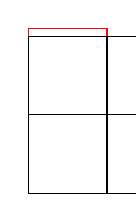
\begin{tikzpicture}
\draw[use as bounding box, red] (0,0) rectangle (1, 2.1);
\draw (0,0) grid +(2,2);
\draw[help lines] (2,0) grid +(2,2);
\end{tikzpicture}

% LOCAL STYLE
\begin{tikzpicture}[help lines/.style={red!50,very thin}]
\path[use as bounding box] (0,0) rectangle (1, 2.5);
\draw (0,0) grid +(2,2);
\draw[help lines] (2,0) grid +(2,2);
\end{tikzpicture}

% APPEND TO STYLE
 %same as black!50,very thin,blue!50, i.e. last one wins.
\begin{tikzpicture}[help lines/.append style=blue!50]
\path[use as bounding box] (0,0) rectangle (1, 2.5);
\draw (0,0) grid +(2,2);
\draw[help lines] (2,0) grid +(2,2);
\end{tikzpicture}

% PARAMETERIZED STYLE
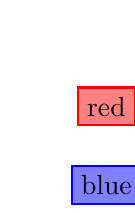
\begin{tikzpicture}[outline/.style={draw=#1,thick,fill=#1!50}]
\path[use as bounding box] (0,0) rectangle (-1, 2);
\node [outline=red] at (0,1) {red};
\node [outline=blue] at (0,0) {blue};
\end{tikzpicture}

%PARAMETERIZED STYLE WITH DEFAULT
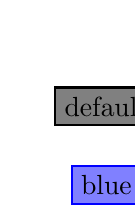
\begin{tikzpicture}[outline/.style={draw=#1,thick,fill=#1!50},
						outline/.default=black]
\path[use as bounding box] (0,0) rectangle (-1, 2);
\node [outline] at (0,1) {default};
\node [outline=blue] at (0,0) {blue};
\end{tikzpicture}

\end{document}
